\documentclass[a4paper,12pt]{report} %togliere quadre per ridurre pagine
\usepackage{graphicx}
\usepackage{hyperref}
\usepackage{placeins}
\usepackage{float}
\usepackage[acronym,nomain,nonumberlist]{glossaries}

\usepackage{titlesec}
\usepackage{enumerate}
\setcounter{tocdepth}{4}
\setcounter{secnumdepth}{4}

\makeatletter
\renewcommand{\thesection}{%
  \ifnum\c@chapter<1 \@arabic\c@section
  \else \thechapter.\@arabic\c@section
  \fi
  \let\Hy@linktoc\Hy@linktoc@none
}
\makeatother

\usepackage{fancyhdr}
\pagestyle{fancy}
\lhead{Marco Rossanese} % controls the left corner of the header
\chead{} % controls the center of the header
\rhead{1177738} % controls the right corner of the header
\lfoot{5G Systems} % controls the left corner of the footer
\cfoot{} % controls the center of the footer
\rfoot{Page~\thepage} % controls the right corner of the footer
\renewcommand{\headrulewidth}{0.4pt}
\renewcommand{\footrulewidth}{0.4pt}


\makeglossaries


\begin{document}
\pagenumbering{gobble}
\clearpage\pagestyle{empty}

\title{

\includegraphics[width=0.4\textwidth]{pics/unipd.jpg}~\\[1.5cm]
NETWORK SLICING OVERVIEW
\\
}

\author{Marco Rossanese 1177738
\\5G Systems - Prof. Stefano Tomasin
\\marco.rossanese@studenti.unipd.it~\\[1cm]
\includegraphics[width=0.4\textwidth]{pics/dei.jpg}
}

\maketitle
\newpage


\tableofcontents
\newpage
\printglossaries
\newpage
%%%%%%%%%%%%%%%%%%%%%%%%%%%%%%%%%%%%%%%%%%%%%%%%%%%%%%%%%%%%%%%%%%%%%%%%%%%%%%%%%%%%%%%%%

% Acronym definitions
\newacronym{sdn}{SDN}{Software Defined Network}
\newacronym{mno}{MNO}{Mobile Network Operators}
\newacronym{ngmn}{NGMN}{Next Generation Mobile Networks}
\newacronym{sil}{SIL}{Service Instance Layer}
\newacronym{nsil}{NSIL}{Network Service Instance Layer}
\newacronym{e2e}{E2E}{End to End}
\newacronym{e2e}{E2E}{End to End}
\newacronym{fh}{FH}{Fronthaul}
\newacronym{bh}{BH}{Backthaul}
\newacronym{CN}{CN}{Core Network}
\newacronym{vi}{VI}{Virtual Infrastructure}
\newacronym{IaaS}{IaaS}{Infrastructure-as-a-Service}
\newacronym{NS}{NS}{Network Services}
\newacronym{VNF}{VNF}{Virtual Network Functions}
\newacronym{MANO}{MANO}{Management and Orchestration}
\newacronym{NBI}{NBI}{Northbound Interface}
\newacronym{SBI}{SBI}{Southbound Interface}
\newacronym{MTA}{MTA}{Multi-Tenancy Application}
\newacronym{NF}{NF}{Network Functions}
\newacronym{CP}{CP}{Control Plane}
\newacronym{UP}{UP}{User Plane}
\newacronym{AN}{AN}{Access Network}
\newacronym{RAT}{RAT}{Radio Access Technology}
\newacronym{NFV}{NFV}{Network Functions Virtualization}
\newacronym{eMBB}{eMBB}{enhanced Mobile Broadband}
\newacronym{mMTC}{mMTC}{massive Machine Type Communications}
\newacronym{URLLC}{URLLC}{Ultra‐Reliable Low‐Latency Communications}
\newacronym{VM}{VM}{Virtual Machines}
\newacronym{InP}{InP}{Infrastructure provider}
\newacronym{ONF}{ONF}{Open Networking Foundation}
\newacronym{SLA}{SLA}{Service Level Agreements}
\newacronym{KPI}{KPI}{Key Performance Indicators}
\newacronym{NFVI}{NFVI}{Network Functions Virtualization Infrastructure}
\newacronym{VIM}{VIM}{Virtual Infrastructure Manager}
\newacronym{VNFM}{VNFM}{Virtual Network Function Manager}
\newacronym{RO}{RO}{Resource Orchestrator}
\newacronym{NSO}{NSO}{Network Service Orchestrator}
\newacronym{NMS}{NMS}{Network Management System}
\newacronym{OSS/BSS}{OSS/BSS}{Operation/Business Support System}
\newacronym{EM}{EM}{Element Management}
\newacronym{IC}{IC}{Infrastructure SDN controller}
\newacronym{TC}{TC}{Tenant SDN controller}
\newacronym{EPC}{EPC}{Evolved Packet Core}
\newacronym{RAN}{RAN}{Radio Access Network}
\newacronym{QoS}{QoS}{Quality of Service}
\newacronym{QoE}{QoE}{Quality of Experience}
\newacronym{RRM}{RRM}{Radio Resource Management}
\newacronym{HSS}{HSS}{Home Subscriber System}
\newacronym{UDM}{UDM}{Unified Data Management}
\newacronym{AUSF}{AUSF}{Authentication Server Functions}
\newacronym{IoT}{IoT}{Internet of Things}
\newacronym{UPF}{UPF}{User Plane Processing Functions}
\newacronym{CPF}{CPF}{Control Plane Processing Functions}
\newacronym{AMF}{AMF}{Access and Mobility Management Function}
\newacronym{SMF}{SMF}{Session Management Function}
\newacronym{UDM}{UDM}{Unified Data Management}
\newacronym{NAS}{NAS}{Non‐Access Stratum}
\newacronym{RRC}{RRC}{Radio Resource Control}
\newacronym{RLC}{RLC}{Radio Link Control}
\newacronym{PDCP}{PDCP}{Packet Data Convergence Protocol}
\newacronym{API}{API}{Application Program Interface}
\newacronym{PCF}{PCF}{Policy Control Function}
\newacronym{NEF}{NEF}{Network Exposure Function}
\newacronym{NRF}{NRF}{NF Repository Function}
\newacronym{N3IWF}{N3IWF}{Non-3GPP InterWorking Function}
\newacronym{UDR}{UDR}{Unified Data Repository}
\newacronym{NSSF}{NSSF}{Network slice selection Function}
\newacronym{AF}{AF}{Application Function}
\newacronym{CSMF}{CSMF}{Communication Service Management Function}
\newacronym{NSMF}{NSMF}{Network Slice Management Function}


%%%%%%%%%%%%%%%%%%%%%%%%%%%%%%%%%%%%%%%%%%%%%%%%%%%%%%%%%%%%%%%%%%%%%%%%%%%%%%%%%%%%%%%%%%%

\newpage
\pagenumbering{arabic}
\setcounter{page}{1}
\pagestyle{fancy}
\section{Introduction}
Mobile networks are a key element of today's society, allowing communication, access
and information sharing. Moreover, traffic forecasts predict that the
demand for capacity will grow exponentially over the next years, this is due mainly to
video services.\\ 
Indeed, since cellular networks move from being voice-centric to
data-centric, telecommunication operators are not able to keep pace with the predicted
increase in traffic volume. Such pressure on operators has
pushed research efforts toward designing 5G novel mobile network solutions
able to open the frontier for new capabilities and revenue sources. In this context, the network
slicing paradigm has emerged as a key 5G technology addressing this challenge.\\
Network slicing for 5G allows \gls{mno} to open
their physical network infrastructure platforms to the concurrent deployment
of multiple logical self-contained networks, orchestrated according
to their specific service requirements; such network slices are then
(temporarily) owned by tenants. The availability of this vertical market\footnote{A vertical market is a group of companies that serve each other's specialized needs and do not serve a broader market, therefore it is mostly focused on meeting the needs of one specific industry.} multiplies
the money incoming opportunities of the network infrastructure as new
opportunities come into play (e.g., automotive industry, e-health) and an higher
infrastructure capacity utilization can be achieved by letting network slice
requests and exploiting multiplexing gains.\\
With network slicing implementations, different services like automotive,
mobile broadband, or tactile Internet can be provided by different network slice
instances: each of these instances consist of a set of virtual network functions
that run on the same infrastructure with a tailored orchestration. In this way,
very different requirements can run on the same infrastructure, as
different network slice instances can be orchestrated and configured separately
according to their specific requirements. Moreover, this is performed in a
cost-efficient manner as the different network slice tenants share the same
physical infrastructure.\\
A network slice is defined by \gls{ngmn} as “\textit{a set of network functions, and
resources to run these network functions, forming a complete instantiated
logical network to meet certain network characteristics required by the Service
Instance(s)}”.\\
According to NGMN, the concept of network slicing involves three layers,
namely:
\begin{enumerate}[1]
\item \gls{sil};
\end{enumerate}
\begin{enumerate}[2]
\item \gls{nsil};
\end{enumerate}
\begin{enumerate}[3]
\item Resource Layer.
\end{enumerate}
The SIL represents the business/end user services furnished by operators or the third party service providers, which are supported by the NISL. The NISL is set of necessary functions to run the instances and the resource layer, which consists of the
resources such as compute, network, memory, storage.\\
The end goal of network slicing in 5G mobile networks is to realize
\gls{e2e} network slices starting from the mobile edge, continuing
through the mobile transport (\gls{fh}/\gls{bh}), and up until
\gls{CN}. The allocation of a slice involves the selection of the
required functions, their constrained placement, the composition of the underlying infrastructure, and the allocation of the resources to fulfill the service's requirements, for example, bandwidth, latency, processing, resiliency.\\
The two main slicing services needed to allow different degrees
of control and management automation in NSIL and resource layers are: the \gls{vi} under the control and operation
of different tenants coherent with an \gls{IaaS} model\footnote{Form of cloud computing that provides virtualized computing resources over the internet} to split information from hardware; \gls{NS} owned by tenants, that is actually creation of a service instance.
The VIs can be operated by the tenant via different \gls{sdn}, NS are instantiated directly over a shared infrastructure
and as a set of interrelated \gls{VNF} connected through
one or more VNF forwarding graphs; both of them will be discussed later.\\
Multi-tenancy is an characteristic that it must be achieved to guarantee separation, isolation, and independence between
different slices coupled with the efficient sharing of the underlying resources
for both VI and NS concepts.\\
\begin{figure}[H]
\centering
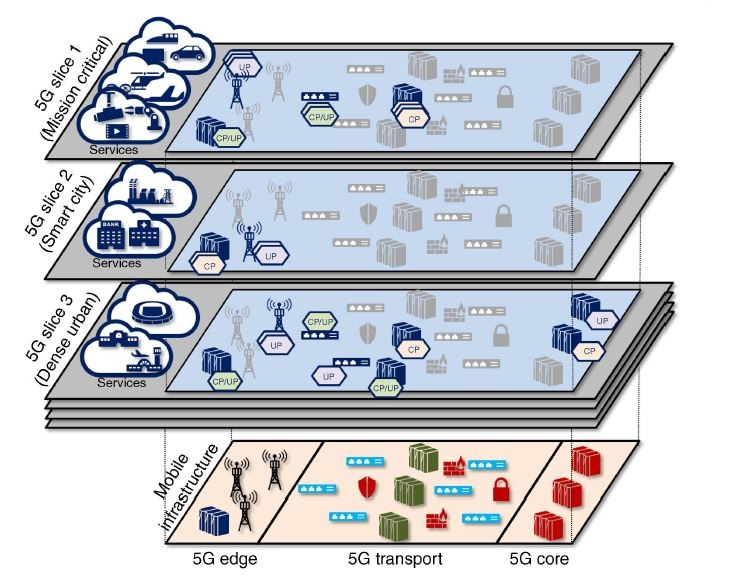
\includegraphics[scale=0.65]{pics/1.JPG}
\caption{Example of network slicing in 5G. \cite{al20185g}}
\label{layers}
\end{figure}
After this general overview this essay will treat accurately all the necessary fundamental components in order to fully understand how 5G network slicing is planned actually to be built.


\newpage
\section{Structural components for Network Slicing} 
Starting from how an architecture for network slicing is conceptually made, it will be explained what it should achieve and involve, that is, the aspects of modularization, resource virtualization, virtual infrastructure and network service management; they will be the main topics of this section.
\begin{figure}[h]
\centering
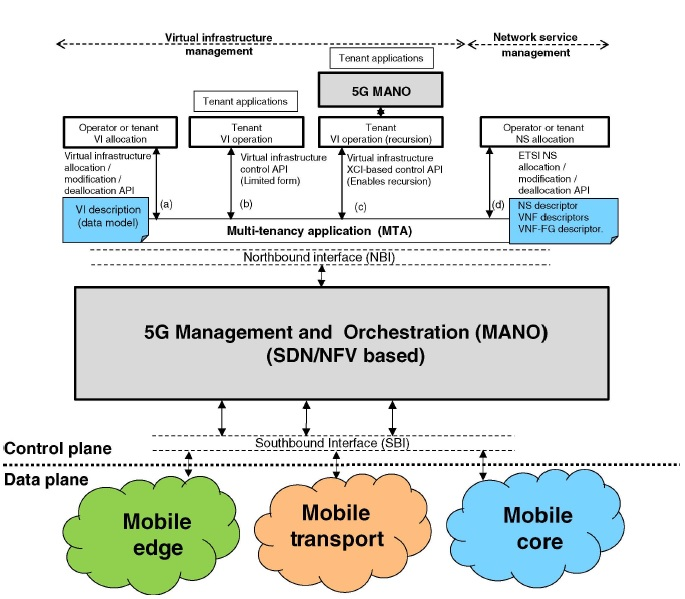
\includegraphics[scale=0.67]{pics/2.JPG}
\caption{Architecture for network slicing. \cite{al20185g}} 
\label{Arch}
\end{figure}
As anticipated about virtualization of the infrastructure, the SDN design is proposed in Fig. \ref{Arch} and follows the principles of:
\begin{itemize}
\item data and control plane fully decoupled;
\end{itemize}
\begin{itemize}
\item control logically centralized;
\end{itemize}
\begin{itemize}
\item applications having an abstracted view of resources and states.
\end{itemize}
The data plane is in practice the resource layer which includes mobile edge, mobile transport, and core. The infrastructure is composed of links, forwarding nodes as switches and routers, cloud nodes  and comprising a set of network, computing, and storage resources.\\
The control plane is divided into two layers: an application layer at the top and the 5G \gls{MANO} platform below. \\
The design of the MANO is based on the ETSI management and network orchestration framework with integrated SDN-based control. The MANO
provides a view of available resources  via a \gls{NBI}, instead it is connected to the data plane
elements via a \gls{SBI} to execute control and management
functions (possible application to do the job are OpenFlow, SNMP, OVSDB) on the actual hardware components.
With respect to the \gls{MTA}, it implements the
multi-tenancy support by coordinating and managing tenants access to a shared
infrastructure, performing resource isolation between instances assigned to
different tenants, and delivering multi-tenancy-related services, such as the
allocation and operation of VIs, by means of dedicated \gls{API}\footnote{An application program interface is code that allows two software programs to communicate with each other.} in cooperation
with the data plane, remarking this logical separation. \\
As shown in Fig. \ref{Arch}
such APIs depend on the actual service: for the control of a VI or NS lifetime,
instantiation, modification, and deletion.

\subsection{Enablers and Design Principles}
Future 5G networks will be built on novel concepts that were not concerned by the previous generation
network architectures. The revolution provided by the introduction of SDN
and \gls{NFV}\footnote{Although NFV and VNF are often used interchangeably, for the sake of clarity NFV is an overarching concept, while a VNF is building block of a NFV framework.} opens the door to a
large list of possible applications recalling that the latter focuses primarily on optimization of the network services, instead the former to separate the control and forwarding plane for a centralized view of the network. The fundamental parts involved in the network slicing realization for the future 5G networks are now discussed.

\subsubsection{Modularization and Function Decomposition}
The evolution of mobile communication systems towards 5G aims at achieving
architecture flexibility, heterogeneous accesses and vertical business integration, exploiting NFV and SDN. The principle of architecture
modularization and network function decomposition was proposed at the earliest 5G research
stages in order to fulfill the above requirements.\\ 
\gls{NF}s are the functional blocks
that provide specific network capabilities to support and realize particular services. Generally implemented
as software instances running on infrastructure
resources, NFs can be physical, that is a combination
of specific hardware and software, or virtualized, that is function service is
decoupled from the hardware it runs on. In particular, conventionally "monolithic" network functions are proposed to be split into basic modules, both for the \gls{CP} and \gls{UP}, allowing the definition of different logical architectures by means of the interconnection of
different subsets of CP and UP NFs.\\
In the process of decomposing the NFs into basic modules, the distinction between NFs relating to
the \gls{AN} and CN emerged. To minimize the dependency of the 5G
core on the access and viceversa and achieve the definition of a convergent network\footnote{Network convergence is the efficient coexistence of telephone, video and data communication within a single network.}, providing
connectivity via a multitude of accesses not only including cellular radio, a different AN/CN functional split and an interface model are necessary.\\
Besides flexibility, the architecture modularization provides the essentials to support network
­slicing, as a network slice can be defined as an independent logical network shaped by the interconnection of a subset of NFs, composing both CP and UP, and which can be independently instantiated
and operated over physical or virtual infrastructure.

\subsubsection{Virtualization}
Virtualization is a key process for network slicing
as it permits effective resource sharing among
slices and it actually is the abstraction of resources
using appropriate techniques. Abstraction means the representation of a resource in terms of
attributes that match predefined selection criteria in order to simplify the its
use and management. \\
The resources to be virtualized can
be physical or already virtualized as well, supporting a
recursive system with different abstraction layers.
Just like server virtualization makes \gls{VM}s independent of the underlying
physical hardware, network virtualization enables
the creation of multiple isolated virtual networks that
are completely decoupled from the underlying physical network and can safely run on top of it.
The framework consists of three kinds of actors:
\begin{itemize}
\item \gls{InP}: owns and manages a given physical network. It offers resources in the form of
WANs or data centers that are virtualized and handed in through programming 
interfaces to a single or multiple tenants.
\end{itemize}
\begin{itemize}
\item Tenant: leases virtual resources from one or
more InPs in the form of a virtual network,
where the tenant can realize, manage, and
provide network services to its users. A network service is a composition of NFs, and it
is defined in terms of the individual NFs and
the mechanism used to connect them.
\end{itemize}
\begin{itemize}
\item End user: consumes the services
supplied by the tenant.
\end{itemize}

\subsubsection{Orchestration}
Orchestration is also a key process for network
slicing and can be
defined as the concept of bringing together and coordinating different things into a coherent whole.
In a slicing environment, where the players involved
are so different, an orchestrator is needed to coordinate heterogeneous network processes for
creating, managing, and delivering services.\\
According to the \gls{ONF},
orchestration is defined as "\textit{the continuing process of
selecting resources to fulfill client service demands
in an optimal manner}". This means to use a policy that governs the orchestrator behavior, which is expected to fulfill all the service level agreements \gls{SLA}s associated with clients
who request services remembering
that the available resources, the service demands, and optimization criteria may change in time. \\
Noteworthy is that orchestration is also referred to as the defining
characteristic of an SDN controller.
However, in network slicing, orchestration cannot be performed by a single centralized entity,
not only because of the complexity, but also because it
is necessary to maintain management independence and support the possibility of recursion. \\
A framework in which each virtualization
actor has an entity performing orchestration functions seems more suitable to satisfy the
above requirements. 

\paragraph{Isolation}\mbox{}\\
Strong isolation is a major requirement that must
be satisfied to operate parallel slices on a common shared underlying substrate. The isolation
must be understood in terms of:
\begin{itemize}
\item Performance: each slice is defined to accomplish particular service requirements, usually expressed in the
form of \gls{KPI}s. Performance isolation is an E2E issue and has to ensure
that service-specific performance requirements are
always met on each slice, regardless of the congestion and performance levels of other slices.
\end{itemize}
\begin{itemize}
\item Security and privacy: attacks or issues occurring in one slice must not affect
other slices. Moreover, each slice must have
independent security functions that prevent unauthorized entities to have read or write access to
slice-specific configuration, management, accounting information.
\end{itemize}
\begin{itemize}
\item Management: each slice must be independently managed as a standalone network.
\end{itemize}
To achieve isolation, a set of appropriate, consistent policies and mechanisms have to be defined
at each virtualization level, following the recursion
principle discussed earlier. The policies contain lists of rules that describe how different entities must be isolated.
To properly realize the required isolation level an team play of both virtualization and orchestration is actually needed.




\subsubsection{SDN: Software-Defined Network}
In a SDN a network engineer can manage traffic from a centralized control console without handling individual switches in the network. The centralized SDN controller directs the switches to deliver network services wherever they are needed, this is actually a move away from traditional network architecture, in which devices make traffic decisions based on their configured routing tables.\\
The SDN architecture comprises, as previously explained and shown in Fig. \ref{layers}, an intermediate control plane is present to dynamically configure and to abstract the underneath forwarding plane resources so as to deliver custom services to clients located in the application plane. This is indeed
well aligned with 5G network
slicing requirements since needs to satisfy a wide range of service demands. Then, the SDN is claimed to be an is an appropriate tool for supporting the key principles of slicing architecture.\\
The main SDN components are resources and controllers. For
SDN, a resource is anything that can be utilized to
provide services in response to client requests, that is infrastructure resources and NFs, but also
network services in application of the recursion
principle described before. A controller is a logically centralized entity instantiated in the control
plane which operates SDN resources at runtime
to deliver services in an optimal way. Therefore,
it finds out tradeoffs among clients and resources, acting simultaneously as server and client via client
and server contexts, respectively. Both contexts
are conceptual components of an SDN controller
enabling the server-client relationships:
\begin{itemize}
\item Client context: represents all the information the
controller needs to handle and transmit to
a given client. It comprises a Resource Group and
a Client support function: the former contains an abstract and customized view of all the resources that the controller offers to the client, through its NBIs, in order to deliver its service demands and ease its interaction
with the controller; the latter instead contains all the
necessary to support client operations, like
policies on what the client is allowed to see and do.
\end{itemize}
\begin{itemize}
\item Server context: represents all the information the controller needs to interact with a set of
underlying resources grouped in a Resource
Group through one of its SBIs.
\end{itemize}
The process of transformation of the Resource Groups set accessed by server contexts to those defined in separate client contexts
is not easy and requires the SDN
controller to perform virtualization and orchestration functions.\\
When performing the virtualization function, the
SDN controller carries out the abstraction and the
aggregation/partitioning of the underlying resources. Thanks to virtualization, each client context provides a specific Resource Group that can be used by the client associated with that context to realize
its services. Through orchestration, the SDN controller distributes in an optimal way the selected resources
to such separate Resource Groups. Thanks to these two functions the fulfillment of the service demands from all clients is guaranteed
while preserving the isolation among them. \\
The SDN architecture also includes an admin whose tasks consist of initializing and configuring the entire controller, including the creation
of both server/client contexts and the selection of their policies.\\
The SDN architecture also supports slicing because the client context provides the complete abstract set of resources as a Resource Group and the supporting control
logic that constitute a slice, including the complete
collection of related client service attributes.\\
Another key aspect that makes SDN
architecture an ideal solution for 5G slicing is recursion. Because of the different abstraction layers
that the recursion principle enables, the SDN
control plane can involve multiple hierarchically
arranged controllers that extend the client-server
relationships at several levels. According to
that, it is clear that SDN can support a
recursive composition of slices. This implies as consequence that
the resources a given controller delivers to one of its clients in the form of a
dedicated slice, i.e. client context, can in turn be
virtualized and orchestrated by such a client in the
case of being an SDN controller. In this way, the new
controller can utilize the resources it accesses via
its server contexts to define, scale, and deliver
new resources and hence new slices to its own
clients, which might also be SDN controllers.


\subsubsection{NFV: Network Functions Virtualization}
Although the SDN architecture described above
gives a comprehensive view of the control plane
functionalities enabling slicing, it lacks capabilities
to efficiently manage the life cycle of
network slices and its resources. \\
VNFs move individual network functions out of dedicated hardware devices into software that runs on commodity hardware. These tasks, used by both network service providers and businesses, include firewalls, domain name system, caching or network address translation and can run as virtual machines. Then, the NFV architecture is ideal to play
this role, as it manages the infrastructure resources
and orchestrates the allocation of such resources
needed to realize VNFs and network services.\\
To benefit from the management and orchestration functionalities of NFV, the right cooperation between SDN and NFV is required.
However, embracing SDN and NFV architectures
into a common reference framework is not an
easy task. ETSI presents a framework
to integrate SDN within the reference NFV architecture. This framework incorporates two SDN
controllers, one logically placed at the tenant and
another at the InP level. The NFV architecture comprises the following
entities:\\
\begin{itemize}
\item \gls{NFVI}: a collection of resources used to
host and connect the VNFs. While SDN makes resource a generic concept,
the current resource definition in the NFV framework comprises only the infrastructure resources.
\end{itemize}
\begin{itemize}
\item VNFs: software-based implementations of NFs that run over the NFVI.
\end{itemize}
\begin{itemize}
\item \gls{MANO}: Performs all the virtualization-specific management, coordination, and automation tasks in the NFV architecture. The MANO framework comprises three functional blocks:
\begin{itemize}
\item \gls{VIM}: responsible for controlling and managing the NFVI resources.
\end{itemize}
\begin{itemize}
\item \gls{VNFM}: performs configuration and life cycle management of the VNF(s) on its domain.
\end{itemize}
\begin{itemize}
\item Orchestrator: according to ETSI, it has two set of functions performed by the Resource \gls{RO} and \gls{NSO}, respectively. The RO orchestrates the NFVI resources across (potentially different) VIMs. The NSO performs the life cycle management of network
services using the capabilities provided by the
RO and the (potentially different) VNFMs.
\end{itemize}
\end{itemize}
\begin{itemize}
\item \gls{NMS}: framework performing the general network management tasks. Although its functions are orthogonal to those defined in MANO, NMS is expected to interact with MANO entities by means of a clear separation of roles. NMS comprises:
\begin{itemize}
\item \gls{EM}: responsible for the configuration,
accounting, performance, and security of a VNF.
\end{itemize}
\begin{itemize}
\item \gls{OSS/BSS}: a collection of systems and management applications that network service providers use to provision and operate their network
services. In terms of the roles we considered
earlier, tenants would run these applications.
\end{itemize}
\end{itemize}
The ETSI proposal includes two SDN controllers
in the architecture. Each controller centralizes
the control plane functionalities and provides an
abstract view of all the components connectivity related it manages. These controllers are:
\begin{itemize}
\item \gls{IC}: sets up
and manages the underlying networking resources to provide the required connectivity for communicating the VNFs.
Managed by the VIM, this controller may change
infrastructure behavior on demand according to
VIM specifications adapted from tenant requests.
\end{itemize}
\begin{itemize}
\item \gls{TC}: instantiated in
the tenant domain as one of the VNFs or as
part of the NMS, this second controller dynamically manages the pertinent VNFs used to realize
the tenant’s network service(s). The operation and management tasks that the
TC carries out are triggered by the applications
running on top of it (e.g. the OSS).
\end{itemize}
Both controllers manage and control their
underlying resources via programmable SBI, implementing protocols like
OpenFlow, NETCONF, and I2RS. However, each
controller provides a different level of abstraction. While the IC provides an underlay to support
the deployment and connectivity of VNFs, the
TC provides an overlay comprising tenant VNFs
that define the network service a tenant independently manages on
its slices. Therefore,
the IC is not aware of the number of slices that utilize the VNFs 
or about the tenants which
operate in the slices. On the other side, for the
TC the network is abstracted in terms of VNFs,
without a knowledge of how those VNFs are physically
deployed. \\
Despite their different abstraction levels,
both controllers have to coordinate and synchronize their actions. Note that the service and
tenant concept mentioned here can be extended
to higher abstraction layers by simply applying the
recursion principle.\\
Finally an overall description of the system is given by Fig. \ref{integral}.
\begin{figure}[h]
\centering
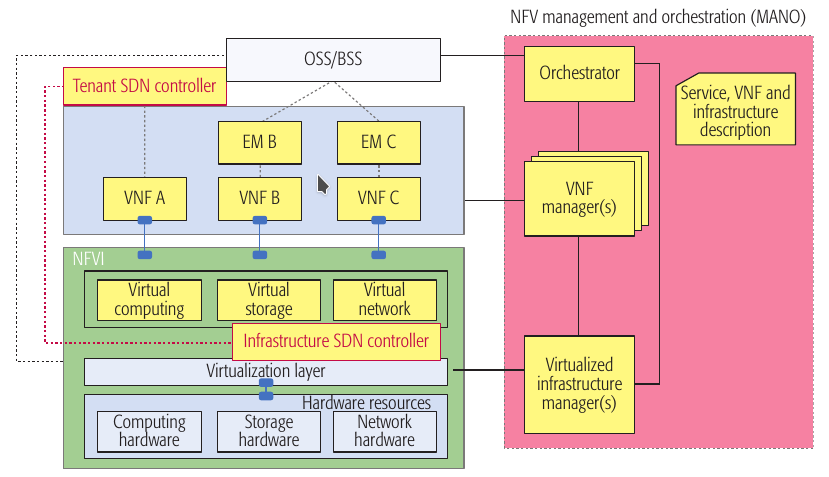
\includegraphics[scale=0.56]{pics/integral.png} 
\caption{Integrating SDN controllers into the reference NFV architectural framework. \cite{ordonez2017network}}
\label{integral}
\end{figure}



\newpage
\section{Network Slicing} 
Now we have all the players to look inside what NGMN has proposed as the concept of network slicing: while legacy systems host multiple telecommunication
services as mobile broadband, voice, SMS on the same mobile network architecture, for
instance composed of Long Term Evolution radio access and the \gls{EPC},
future 5G networks should also support shared or dedicated logical architectures customized to the
respective telco or vertical services as \gls{eMBB}, vehicular communications, \gls{URLLC}, and \gls{mMTC}. These services need different KPIs that are
hard to be fulfilled by legacy systems which are characterized by monolithic network elements that
have tightly coupled hardware, software, and functionality. \\
Future architectures must leverage on the decoupling of software‐based network functions from the underlying infrastructure resources by
means of utilizing different resource abstraction technologies.
Furthermore exploiting modularization, resource sharing technologies such as multiplexing and multitasking (for instance
wavelength division multiplexing or radio scheduling), can be complemented
by softwarization techniques. Multitasking and multiplexing allow sharing
physical infrastructure that is not virtualized. NFV and SDN allow different tenants to share the
same general purpose hardwares. 
\begin{figure}[H]
\centering
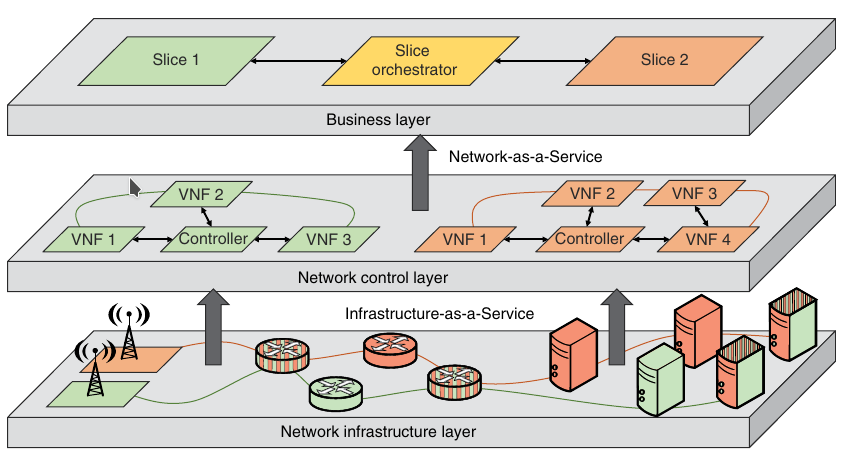
\includegraphics[scale=0.55]{pics/slice.png}
\caption{An example of a network‐sliced architecture. \cite{al20185g}} 
\label{slice}
\end{figure}
In combination, these technologies allow building fully decoupled E2E networks on top of a common, shared infrastructure and consequently, multiplexing will not be done on the network level anymore, but on the
infrastructure level, as depicted in Fig. \ref{slice}, yielding better \gls{QoS} or \gls{QoE} for the subscriber since different slices will have tailored orchestration for a given
servic.\\
In principle, a network slice is a logical network that provides specific network capabilities and
network characteristics and comprises NFs, computing and networking resources to meet the
­performance requirements of the tenants. This comprises both \gls{RAN} and CN NFs that depending on the degree of freedom a tenant may have, also
the MANO components. A network slice may be dedicated to a
specific tenant or partially shared by several tenants in order to have the same performance requirements
but different security or policy settings. \\
The decoupling between the virtualized and the physical
infrastructure allows for the efficient scaling of the slices, hence suggesting the
economic viability of this approach that can adapt the used resources on demand.\\
The 5G atom proposed in Fig. \ref{atom} summarizes the discussion: use cases are in the center; the layers, from the center out, represent the requirements of the 5G use cases, the concepts that will allow network
operators to satisfy the requirements, the technologies that enable the implementation of
the concepts, and the novelties, that is, technologies that can be easily implemented due
to softwarization and virtualization techniques.
\begin{figure}[h]
\centering
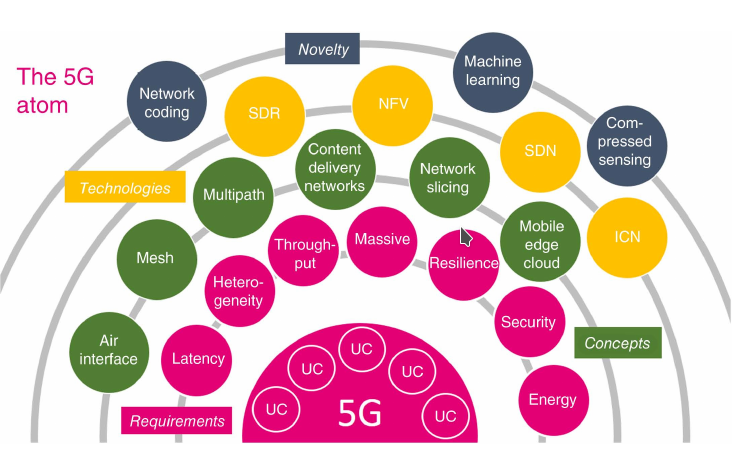
\includegraphics[scale=0.63]{pics/5g_atom.png} 
\caption{5G atom representation. \cite{marsch20185g}}
\label{atom}
\end{figure}


\subsection{Main Services Types}
The main 5G service types typically considered are:
\begin{itemize}
\item Enhanced mobile broadband (eMBB): related to human operations and to an enhanced access to multimedia content, services and data with improved performance with an increasing user experience. This service type, which can be seen as an evolution of the services today provided by
4G networks, covers use cases with very different requirements, ranging from hotspot characterized by a high user density and very high traffic capacity and low user mobility, to wide area coverage cases with medium to high user mobility; besides the need for seamless radio coverage practically
anywhere and anytime with visibly is requested to improve user data rates;
\end{itemize}
\begin{itemize}
\item Ultra‐reliable and low-latency communications (URLLC): related to use cases with tight requirements for capabilities such as latency, reliability and availability. Examples include the wireless
control of industrial manufacturing or production processes, remote medical surgery, distribution automation in a smart grid, transportation safety, etc. It is expected that URLLC services will provide a main part of the foundations for the 4th industrial revolution (often referred to as
Industry 4.0) and have a substantial impact on industries far beyond the information and communication technology industry;
\end{itemize}
\begin{itemize}
\item Massive machine‐type communications (mMTC): capturing services that are characterized by
a very large number of connected devices typically transmitting a relatively low volume of non delay sensitive data. However, the key challenge is here that devices are usually required to be
low-cost, and have a very long battery lifetime. Key examples for this service type would be logistics applications, smart metering, or for instance
agricultural applications where small, low‐cost and low‐power sensors are sprinkled over large
areas to measure ground humidity, fertility and what concerns Intern of Things in general.
\end{itemize}
The concept of network slicing will be implemented at the beginning of the 5G era in order to realize these main services as slices and their 8 most important KPI are the following:
\begin{itemize}
\item Peak data rate, referring to the maximum achievable data rate in ideal conditions per user or
device in bits per second. The minimum 5G requirements for peak data rate are 20 Gbps in the
downlink and 10 Gbps in the uplink;
\end{itemize}
\begin{itemize}
\item User experienced data rate, referring to the achievable data rate that is available ubiquitously
across the coverage area to a mobile user or device in bits per second. This KPI corresponds to the
5\% point of the cumulative distribution function of the user throughput and can be seen as
a kind of minimum user experience in the coverage area. This requirement is set to
100 Mbps in the DL and 50 Mbps in the UL;
\end{itemize}
\begin{itemize}
\item Average spectral efficiency, also known as spectrum efficiency and defined as the average data
throughput per unit of spectrum resource and per cell in bps/Hz/cell. Again, the minimum requirements depend on the test environments as follows:
\begin{itemize}
\item Indoor Hotspot: 9 bps/Hz/cell in the DL, 6.75 bps/Hz/cell in the UL;
\end{itemize}
\begin{itemize}
\item Dense Urban: 7.8 bps/Hz/cell in the DL, 5.4 bps/Hz/cell in the UL;
\end{itemize}
\begin{itemize}
\item Rural: 3.3 bps/Hz/cell in the DL, 1.6 bps/Hz/cell in the UL.
\end{itemize}
\end{itemize}
\begin{itemize}
\item Area traffic capacity, defined as the total traffic throughput served per geographic area in Mbps/m2, defined only for the indoor hotspot case, with a target of 10 Mbps/m$^2$ for
the downlink;
\end{itemize}
\begin{itemize}
\item User plane latency, that is the contribution of the radio network to the time from when the
source sends a packet to when the destination receives it and the latency
requirement is set to 4 ms for eMBB services and 1 ms for URLLC;
\end{itemize}
\begin{itemize}
\item Connection density, corresponding to the total number of connected 
per unit area, targeting 1000000 devices per km$^2$ for mMTC services;
\end{itemize}
\begin{itemize}
\item Energy efficiency, refers to the quantity of information bits transmitted to or received from users, per unit of energy consumption of the RAN and on the device side to the
quantity of information bits per unit of energy consumption of the communication module; both cases in bits/Joule. Air interfaces must have the capability to support a high sleep ratio and long sleep duration;
\end{itemize}
\begin{itemize}
\item Mobility, here defined as the maximum speed at which a defined QoS and
seamless transfer between radio nodes which may belong to different layers or radio access
technologies can be achieved. For the rural test environment, the normalized traffic channel link
data rate at 500 km/h, reflecting the average user spectral efficiency, must be larger than 0.45 bps/Hz
in the uplink.
\end{itemize}
The following web-spider diagrams in Fig. \ref{cap1}-\ref{cap2}, sum up optimally these capabilities and how they have to be split to realize each particular slice
\begin{figure}[h]
\centering
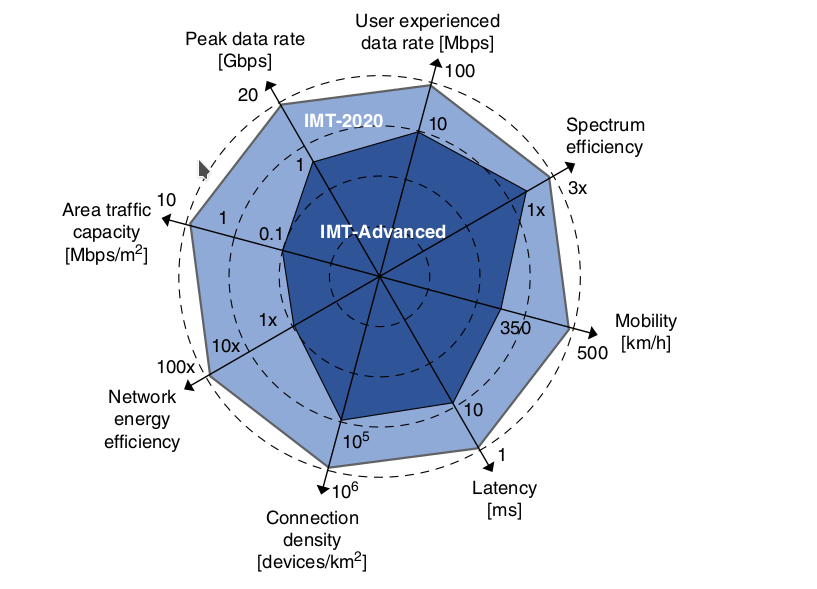
\includegraphics[scale=0.4]{pics/capabilities1.png}
\caption{Capabilities to be achieved. \cite{al20185g}} 
\label{cap1}
\end{figure}
\begin{figure}[H]
\centering
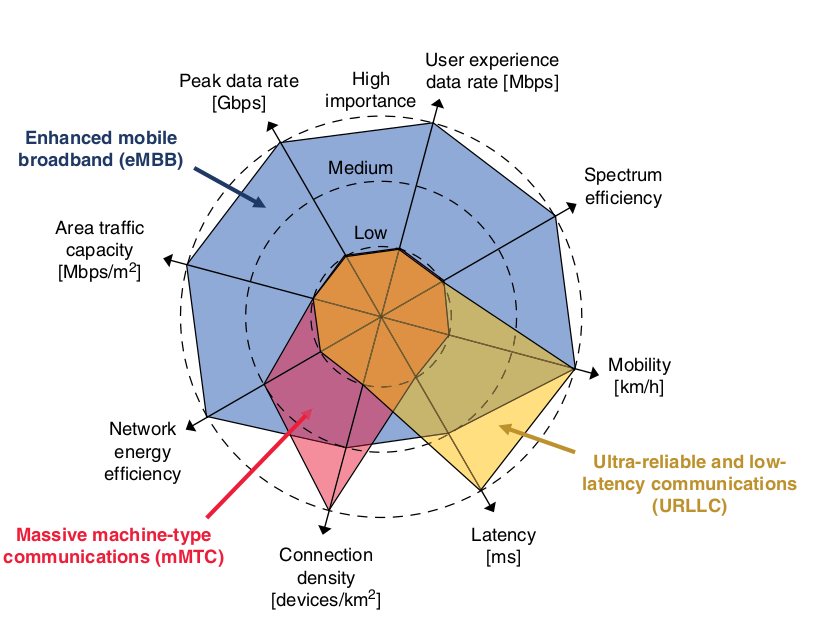
\includegraphics[scale=0.4]{pics/capabilities2.png}
\caption{How capabilities are divided for each slice. \cite{al20185g}} 
\label{cap2}
\end{figure}




\newpage
\section{5G Architecture}
3GPP has split 5G specifications in
two phases: the first called Release-15 and released on August 2018 addressing
a urgent subset of commercial
needs; the second, called Release-16 is planned to be completed by March
2020 addressing all identified use cases and
requirements. 
Now, by giving a look at Release-15 a representation of 5G architecuture is illustrated in order to understand how the novel concept of netowork slicing is implemented; Fig. \ref{archite}
\begin{figure}[h]
\centering
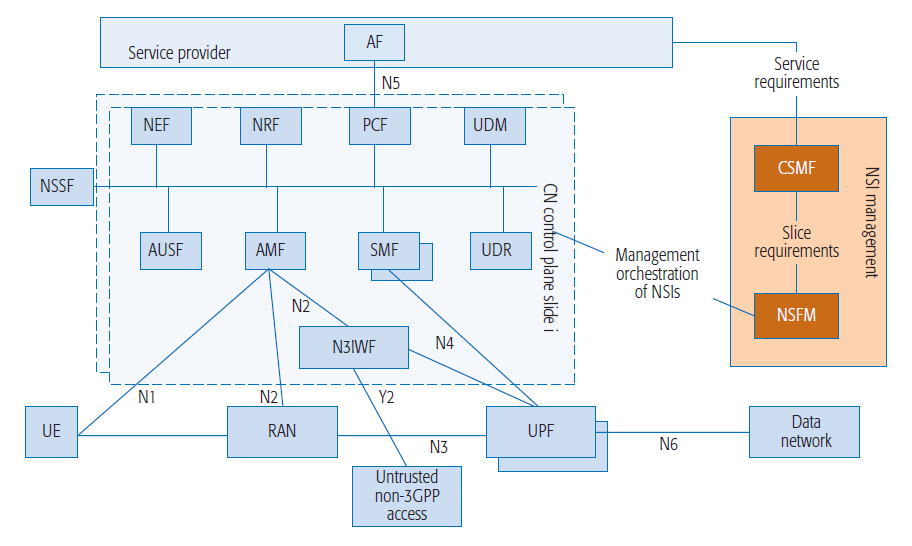
\includegraphics[scale=.57]{pics/5g_architecture.PNG}
\caption{5G System architecture. \cite{etsi2018gs} \cite{kaloxylos2018survey}}
\label{archite}
\end{figure}
Compared to the LTE architecture, 3GPP
has decided to modularize mainly the CN
and allocate slice-related NFs inside it. The CN
control plane functions are now described:
\begin{itemize}
\item Core access and mobility management function
(AMF) necessaru mobility management, access
authentication and authorization, security
anchor functions and context management;

\item Session management function (SMF) handles session
management, IP address allocation, traffic
steering, selection and control of UP functions,
control part of policy enforcement,
and QoS;

\item \gls{PCF} specifies an unified policy
framework to govern network behavior and policy
rules to control plane functions;

\item \gls{NEF} provides
to securely expose the services and
capabilities provided by NFs;

\item \gls{NRF} is a service discovery
function used by NF instances;

\item Unified data management (UDM) concerns the authentication
credential repository and processing
function, user identification handling, subscription
management;

\item Authentication server function (AUSF): supports
the authentication server;

\item \gls{N3IWF} is necessary to support:
IPsec tunnel establishment, relay signaling
between user equipment and AMF,
relay user plane packets between UE and UPF, anchor point within non-3GPP access networks;

\item \gls{UDR} stores subscription
and policy data;
\end{itemize}
The architecture also contains the following
functions:
\begin{itemize}
\item User plane function (UPF) is an anchor point for
inter/intra-radio access technology
mobility and necessary for packet routing and forwarding,
QoS handling for the user plane;

\item \gls{NSSF} supports
the functionality to bind a user equipment with a
specific slice;

\item \gls{AF} influences traffic
routing, accesses the NEF, interacts with PCF;
\end{itemize}
5G allows user equipments to concurrently
access multiple
network slices concurrently, but in such a
case, only a single AMF will be used for all slices.
It has been agreed that they cannot use more
than eight slices in parallel.
To identify slices, the network slice selection assistance
information is used and consists of
the slice/service type, an entity which identifies the
NFs a slice provides. 3GPP has
standardized 3 slice/service type values,one for eMBB,
2 for URLLC and 3 for MIoT. Therefore, CN
is responsible to authorize the attachment of UE
to a slice.
The management functions for network
slices are called \gls{CSMF} and \gls{NSMF}. The CSMF is used
to translate the communication service requirements
to network slice requirements (capacity,
throughput, delay, number of users, geographical
identifications, authentication level). The
NSMF is responsible for managing and orchestrating
the life cycle of a network slice. This life cycle
consists of the following phases:
\begin{itemize}
\item Preparation phase;

\item Instantiation, configuration, and activation
phase;

\item Runtime phase;

\item Decommissioning phase;

\end{itemize}
The first phase involves the creation and verification
of a slice template. During the second phase,
all shared or dedicated NFs and resources are
allocated and configured. During the third phase,
a network slice is essentially a fully operational
network, and monitoring and optimization functions
are also performed. The last phase is related
to the deactivation of a slice and the decommissioning
of previously allocated resources.



\newpage
\section{Actual Implementations}
Some early trials have been conducted demonstrating network slicing with
cross-industry collaboration among operators, vendors, and vertical industries.
Two specific examples are given here.
\begin{itemize}
\item Deutsche Telekom and Huawei demonstration of E2E autonomous network slicing. In this demo, eMBB, mMTC and uRLLC are envisaged as network classes that could be built as slices.
E2E network slicing included not only the core network and RAN, but also
interconnecting transport networks. The demo implements E2E network slicing automation based on service oriented network auto creation. It uses software-defined topology, software-defined protocol, and
software-defined resource allocation to ensure the automatic implementation of slice management, service deployment, resource scheduling, and fault recovery.
\end{itemize}
\begin{itemize}
\item SK Telecom, Deutsche Telekom and Ericsson have jointly built
and demonstrated a trial network on federated network slicing for roaming, making SK Telecom and DT network slices available in each operators footprint, connecting South Korea and Germany. The demonstration
was hosted at Deutsche Telekom's corporate R\&D center in Bonn, Germany and Sk Telecoms 5G testbed at Yeongjongdo (the BMW driving center) in Korea. The
demo featured an industrial maintenance use case involving a repair worker
communicating via augmented reality with support colleagues in a visited network. The scenario used local breakout and edge cloud to enable
the best service experience in terms of latency and throughput for the augmented reality
repairman.
\end{itemize}


\phantomsection 
\addcontentsline{toc}{chapter}{Bibliography} 

\newpage
\nocite*
\bibliographystyle{plain}
\bibliography{biblist}

\end{document}